

In this section, we present and analyze the obtained results from the experimental evaluation of the devised decentralized aggregation protocol when compared with a popular monitoring solution from the state-of-the-art: named Prometheus~\cite{prometheus}. We begin by providing the experimental setting and configuration settings used across the conducted experiments, then we present and discuss the obtained results from these experiments, and finish the Section by providing a summary along with the drawn conclusions from the evaluation of our solution in its monitoring and aggregation capacity.

The experimental setting in which the evaluation of our aggregation protocol was conducted on is the same as the one defined in~\ref{sec:exp_setting_conf}, where each solution is tested using containers to multiplex the physical nodes, isolate the running processes, and apply both bandwidth capacity constraints and latency delays between nodes.

As previously mentioned in Section~\ref{sec:mon_protocol}, the devised aggregation protocol offers three decentralized information collection primitives: neighbourhood, tree and global aggregation. In this section, we provide the obtained results regarding the evaluation of the tree and global aggregation features with comparable setups running Prometheus. Neighbourhood aggregation results are not shown as Prometheus does not provide a comparable feature (which we believe is already a result in itself). For all the conducted experiments, we tested the systems by collecting a certain aggregated value, calculated through the aggregation of a variable number of metrics, emitted at configurable intervals by dummy applications running in all the nodes of the system. The main criteria used to test the applicability of our solution was its error over time: obtained by comparing the aggregated value obtained by each node against their ``supposed'' value, according to the following formula: 

\[ Error(t) =  \frac{|\sum localVal_i(t) - aggVal(t)|}{\sum localVal_i(t)}\]

Where $localVal_i$ corresponds to the emitted value of each node locally, $\sum localVal_i$ corresponds to the ``real'' value, and $aggVal$ corresponds to the obtained aggregated value during the experiment. In addition to the error over time, we collected other metrics to measure the performance of our solutions, such as the consumption of networking and computing resources. All tests were conducted with network sizes of 750 logical nodes, and for each experiment, we varied the number of metrics emitted by the dummy applications. Finally, for each of these experiment combinations, we conducted tests with failure rates of 0 and 50\% of the nodes in the system, excluding the configurated tree roots.

The designed features were compared against Prometheus configured in two, distinct, tree-shaped setups: the first setup, which we named \textbf{centralized Prometheus}, corresponds to the most typical configuration of a Prometheus server, where a single server collects and aggregates the metrics correspondent to all the nodes in the system. The second experimental setup, named \textbf{Prometheus tree}, corresponds to a more sophisticated setup where instead of having a single aggregating node, there is an intermediate layer of nodes aggregating the metric values of the leaf nodes. This intermediate layer, in turn, is aggregated by the root node (effectively splitting the load among the aggregator nodes). The root node, in this configuration, makes use of ``federation'' to scrape the partially aggregated value from the Prometheus servers in the intermediate layer.

In the following reported experiments, there are two parameters displayed for the Prometheus results, the first, denoted by $i$, corresponds to the size of the intermediate layer, the second parameter, denoted by $o$, corresponds to the number of servers to aggregate for each node in the intermediate layer (essentially, $o$ corresponds to maximum number of leaf nodes in the Prometheus deployment). In addition, for both of the centralized and tree configurations, we also test setup a variation where every node in the system is an aggregator node (with the name \textbf{aggregator leaves}), which aggregates the metrics provided by their local dummy application and only export the aggregated value. It is important to mention that only the first two setups (centralized and tree) are, to our knowledge, the most representative of common Prometheus configurations, however, we include the aggregator leaves scenarios to study the impact in terms of network cost of performing in-transit aggregation by every node which emits metrics when compared to performing the aggregation process of metrics extracted from multiple nodes by a single node. An illustration of these setups can be found in Figure~\ref{fig:sec:eval_prom_setups}.

\begin{figure}
    \centering
    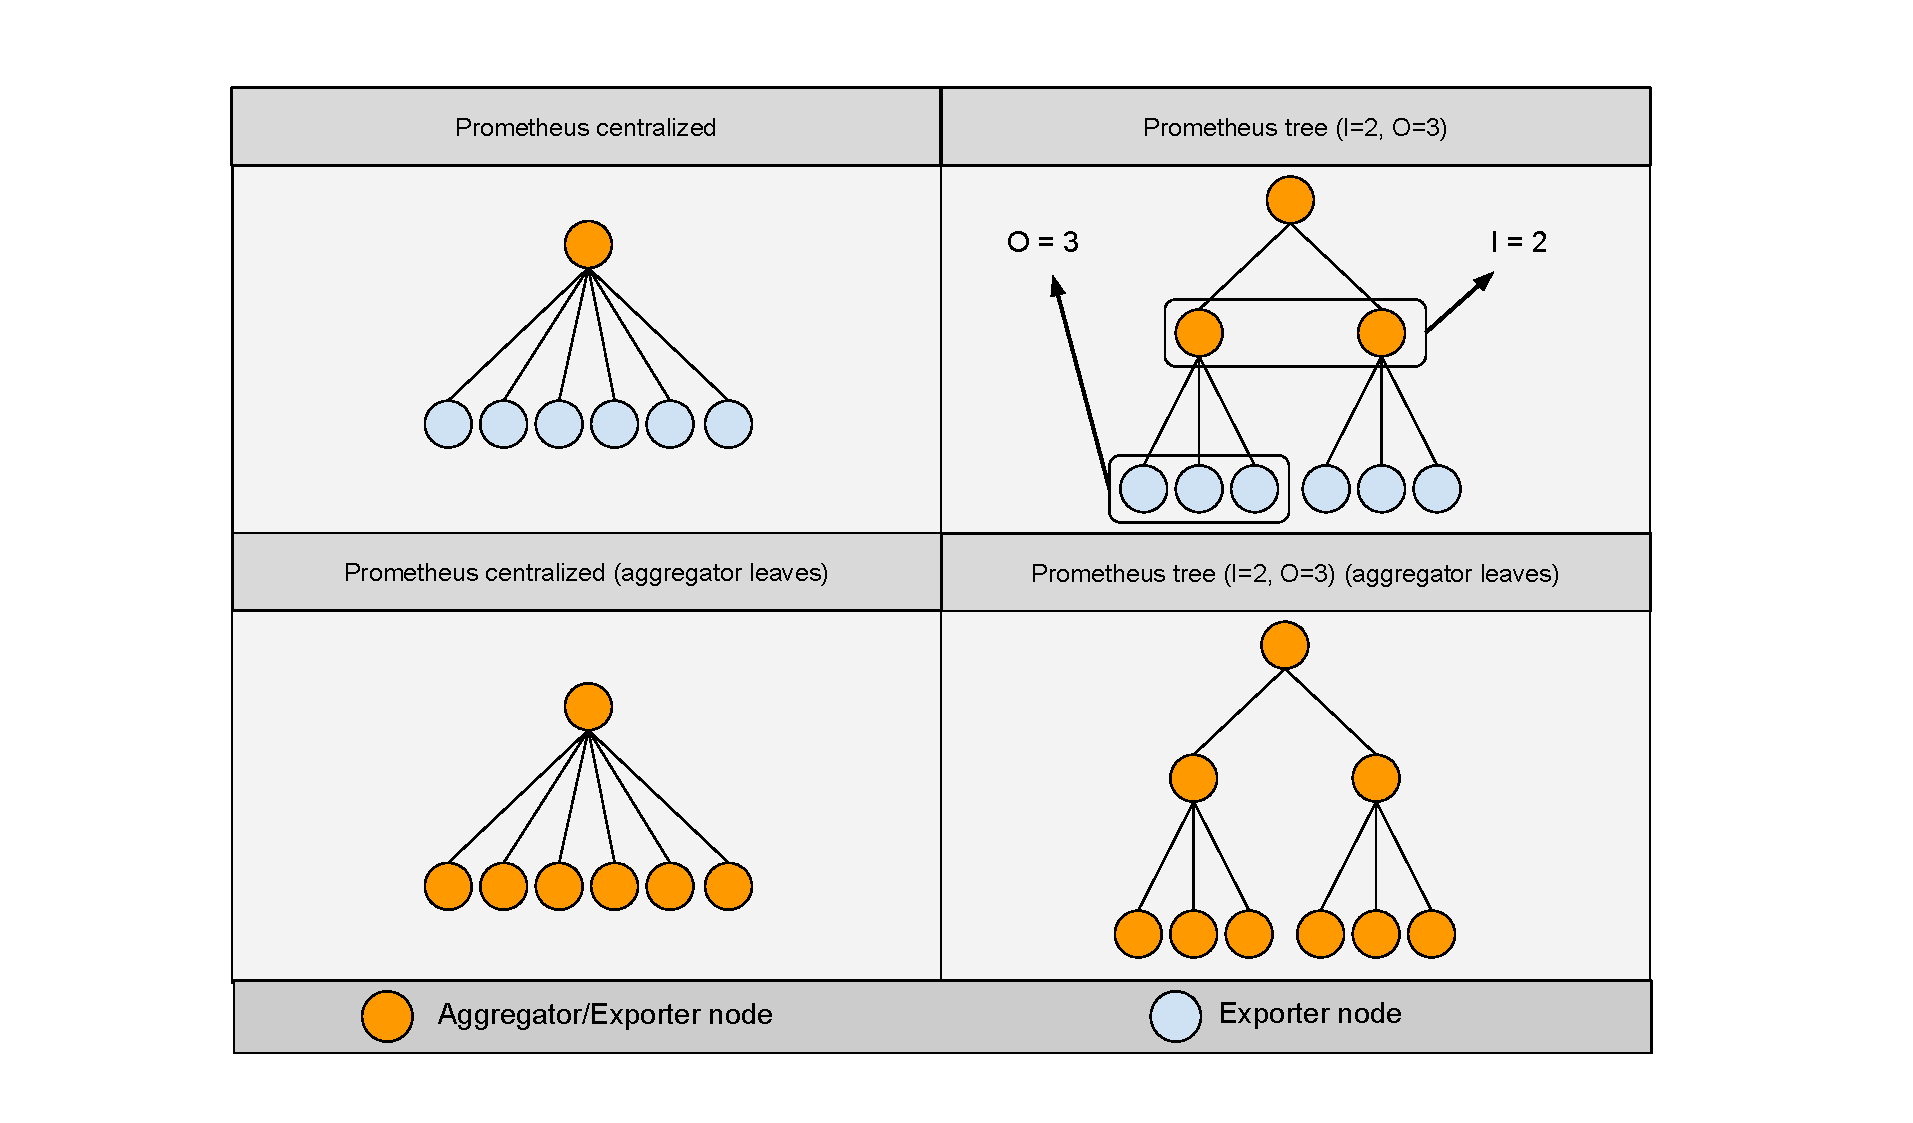
\includegraphics[width=\linewidth]{Chapters/evaluation/figures/aggregation/Prometheus setups.pdf}
    \caption{Exemplification (at smaller scale) the of tested prometheus setups}
    \label{fig:sec:eval_prom_setups}
\end{figure}

\subsection{Tree aggregation}

For the \textbf{tree aggregation} evaluation, we configured DeMMon with a single tree aggregation function, which triggers the algorithm defined in Section~\ref{sec:mon_protocol} that, in summary, collects an aggregated value of the metrics of its descendants in the DeMMon tree. This feature was designed for decentralized resource management applications that follow the DeMMon hierarchical structure to perform decentralized resource management decisions. For example, a certain application that wishes to maintain a certain ratio of two service replicas (because one depends on the other), can do so by having each node monitor its descendants and perform resource management actions (possibly coordinated with other nodes) to replenish or decommission a service replica such that the desired ratio is maintained.

To test this feature, we set up both Prometheus and DeMMon collecting an aggregated value of the whole system in a single node, providing an aggregated view of the system (in our case, we used the sum to produce the aggregated value), and collected the error of the obtained aggregated value against the correct value over time. In addition to the error, we also collected the total network cost over the duration of the experiments. 

\begin{figure}
    \centering
    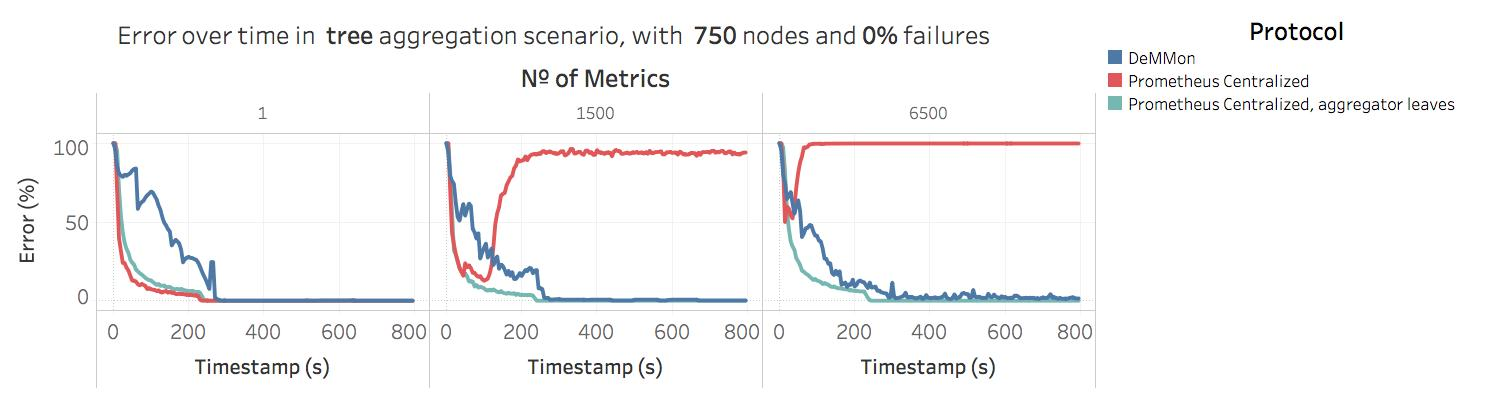
\includegraphics[width=\linewidth]{Chapters/evaluation/figures/aggregation/Error_over_time_tree_0_failures_centralized.jpg}
    \caption{Error over time obtained in tree aggregation (centralized scenario)}
    \label{fig:sec:mon_eval_tree_centralized}
\end{figure}

We begin this comparison by discussing the obtained results regarding the centralized version of Prometheus against DeMMon (Figure~\ref{fig:sec:mon_eval_tree_centralized}), where we may observe that both DeMMon and Prometheus reach the 0\% error values across all conducted tests, which means the systems are working correctly. Furthermore, we may observe that, in the regular Prometheus setup (non-aggregator leaves), as the number of metrics increases, Prometheus cannot obtain the metrics to calculate the aggregated value. We believe this occurs because the root node exceeds its allocated bandwidth. This contrasts with the Prometheus ``aggregator leaves'' results, which obtain 0\% error value across all conducted experiments, which happens because every node is aggregating their emitted metrics and only propagating an aggregated value, which does not saturate the system bandwidth. It is important to notice that as the number of series increases, the DeMMon error tends to fluctuate between 0 and low error values. We believe this occurs due to the DeMMon nodes saturating their CPU when parsing the metrics. Although we realize this may be a limitation of the developed system, we argue this limitation is an engineering problem that may be easily addressed by employing a more efficient metric transmission and parsing protocol (similar to Prometheus' or InfluxDBs'~\cite{influxdb_data_elements}).

\begin{figure}
    \centering
    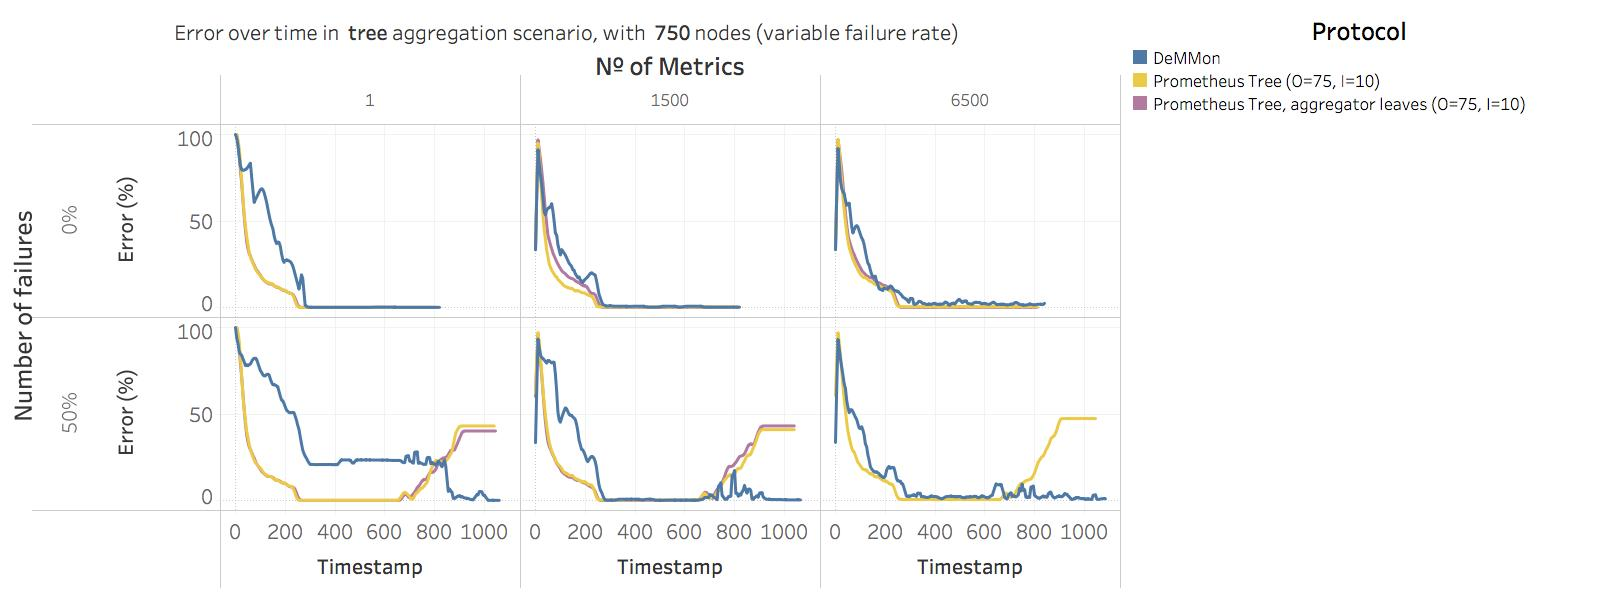
\includegraphics[width=\linewidth]{Chapters/evaluation/figures/aggregation/Error_over_time_tree_tree.jpg}
    \caption{Error over time obtained in tree aggregation (tree scenario)}
    \label{fig:sec:mon_eval_tree_tree}
\end{figure}

As the centralized Prometheus setup saturates at higher metric counts, we now compare the performance of our solution against a more scalable Prometheus setup, the \textbf{Prometheus tree} setup. The results of this comparison may be observed in Figure~\ref{fig:sec:mon_eval_tree_tree}, which contains the error over time obtained for the experiments with 0\% and 50\% failure rates. As we can observe, Prometheus (in the non-aggregator leaves scenario) now splits the load of aggregating the metrics throughout multiple nodes and consequently can obtain the correct aggregated value. This configuration, however, is plagued by multiple unrecoverable points of failure, this is shown in the scenarios with 50\% failures (bottom half of the graph), where Prometheus setups do not recover from the induced failures, as servers require manual intervention to change their configuration to surpass the effect of such failures.

\begin{figure}
    \centering
    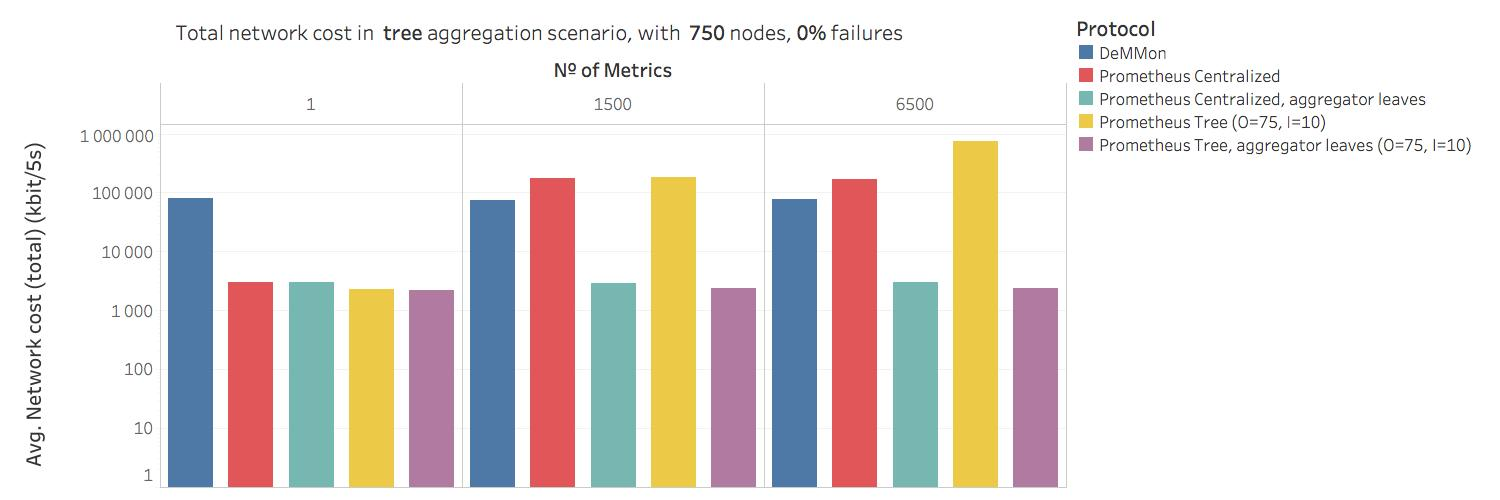
\includegraphics[width=\linewidth]{Chapters/evaluation/figures/aggregation/network_cost_tree.jpg}
    \caption{Average network cost incurred during tree aggregation experiments}
    \label{fig:sec:mon_eval_tree_net_cost}
\end{figure}

Finally, in Figure~\ref{fig:sec:mon_eval_tree_net_cost}, we can observe the average network cost for the previously shown experiments. In this graph, we can observe that the ``aggregator leaves'' incur a constant cost number, which is also the lowest obtained result when compared with other setups. This is expected because these setups perform aggregation of their metrics locally before emitting them towards the root node. In the case of DeMMon, the incurred networking cost is also constant, as DeMMon also performs local aggregation before emitting the results. In the case that we believe to be the most representative Prometheus deployments, the network costs tend to increase linearly with the number of metrics, which is less desirable when compared to a constant networking cost.

\subsection{Global aggregation}

Global aggregation in DeMMon (as further explained in Section~\ref{sec:mon_protocol:global_agg}) is a feature where each node in the system calculates the result of the aggregation in a decentralized manner. To test the applicability of this feature, we also employed Prometheus as a baseline comparison, also configured in the same way as described at the beginning of this section. However, for fairness in the comparison, we configured each Prometheus server to node periodically query the root node for obtaining the aggregated value (effectively providing the same results as DeMMon).

\begin{figure}
    \centering
    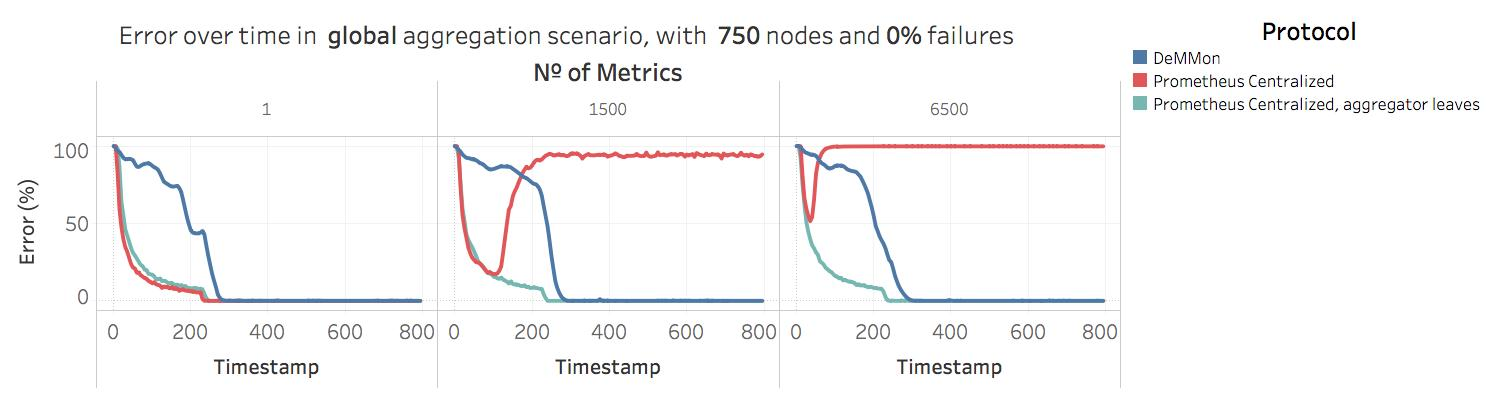
\includegraphics[width=\linewidth]{Chapters/evaluation/figures/aggregation/Error_over_time_global_0_failures_centralized.jpg}
    \caption{Error over time obtained in global aggregation (centralized scenario)}
    \label{fig:sec:mon_eval_global_centralized}
\end{figure}

\begin{figure}
    \centering
    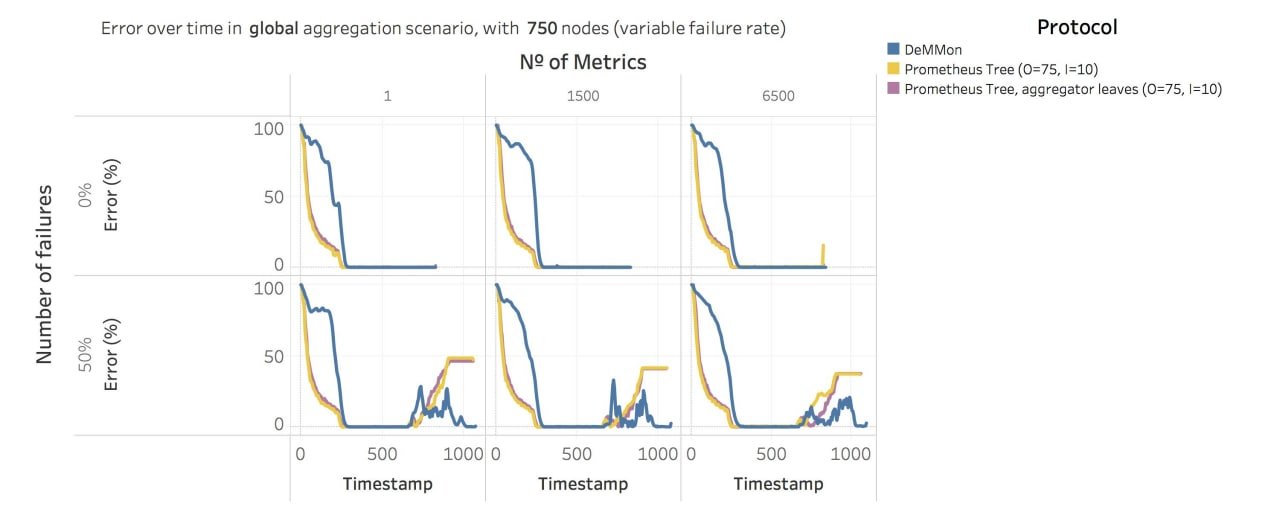
\includegraphics[width=\linewidth]{Chapters/evaluation/figures/aggregation/Error_over_time_global_tree.jpeg}
    \caption{Error over time obtained in global aggregation (tree scenario)}
    \label{fig:sec:mon_eval_global_tree}
\end{figure}

The experiments conducted for this feature are similar, in terms of duration and failure rate, to the ones conducted for tree aggregation. Their results can be observed in Figures~\ref{fig:sec:mon_eval_global_centralized} and~\ref{fig:sec:mon_eval_global_tree}. In these, we note a similar pattern to the one observed by the tree aggregation results, namely: the centralized Prometheus configurations cannot scale when the number of metrics emitted per node increases, and the tree Prometheus configurations, while they mitigate the scaling problem, are subjected to multiple points of failure that, in the case of a failure, require manual configuration to recover. 

Finally, in these results, we may observe that DeMMon can correctly obtain the aggregated value even when the number of metrics increases, even the presence of failures, making it a more versatile option for scenarios where failures are common, such as those found at the edge of the network.

\begin{figure}
    \centering
    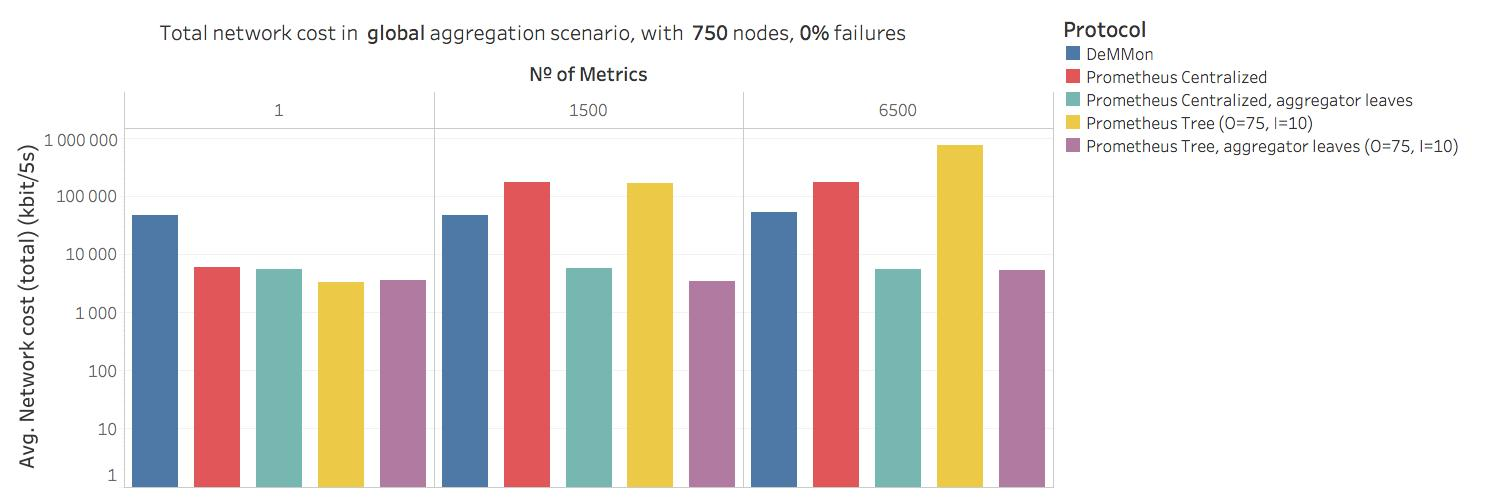
\includegraphics[width=\linewidth]{Chapters/evaluation/figures/aggregation/network_cost_global.jpg}
    \caption{Average network cost incurred during global aggregation}
    \label{fig:sec:mon_eval_global_net_cost}
\end{figure}

The final experimental result, showing the average network cost incurred during these experiments, can be observed in Figure~\ref{fig:sec:mon_eval_global_net_cost}, where similarly to tree aggregation, both DeMMon and the two Prometheus configurations with ``aggregator leaves'' obtain constant network costs during the experiments (because these setups perform local aggregation before emitting their metrics). Furthermore, these Prometheus setups incur less networking costs, given they do not have to maintain the overlay network, unlike DeMMon. 

The remaining configurations (Prometheus tree and Prometheus centralized), as they do not perform in-transit aggregation of the metrics, incur networking costs that scale with the number of metrics emitted by the nodes. Consequently, from the standpoint of scalability, this means the scalability of such deployment will be limited by the number of series emitted per node, that contrary to DeMMon or configurations with ``aggregator leaves'' (which as previously mentioned, are not representative of most Prometheus setups), achieve linear networking costs with the number of emitted metrics.

